\documentclass[a6paper,11pt]{article}
%\usepackage[T1]{fontenc}
\usepackage[british]{babel}
\usepackage[utf8]{inputenc}
\usepackage{float, graphicx,amsmath,amsfonts,cite,enumerate}
\usepackage[final]{pdfpages}
\usepackage{wrapfig}
\usepackage[margin=0.3in]{geometry}
%\usepackage{sidspaltHack} % Not used to make room for phi
\usepackage{digital}


\setlength{\oddsidemargin}{-0.47in}
\setlength{\textwidth}{235pt}

\pagestyle{empty}
\renewcommand{\songtitle}[2]{\Large{#1. #2}\\\small} % Add small to the command

\begin{document}
\newpage
\chaptertitle{$\Omega\omega$}{Noter}
\vspace{-5pt}\small
\begin{center}
\songtitle{$\omega1$}{Du gamla du fria}
\end{center}
\vspace{-40pt}
\begin{figure}[!h]
\hspace{-10pt}
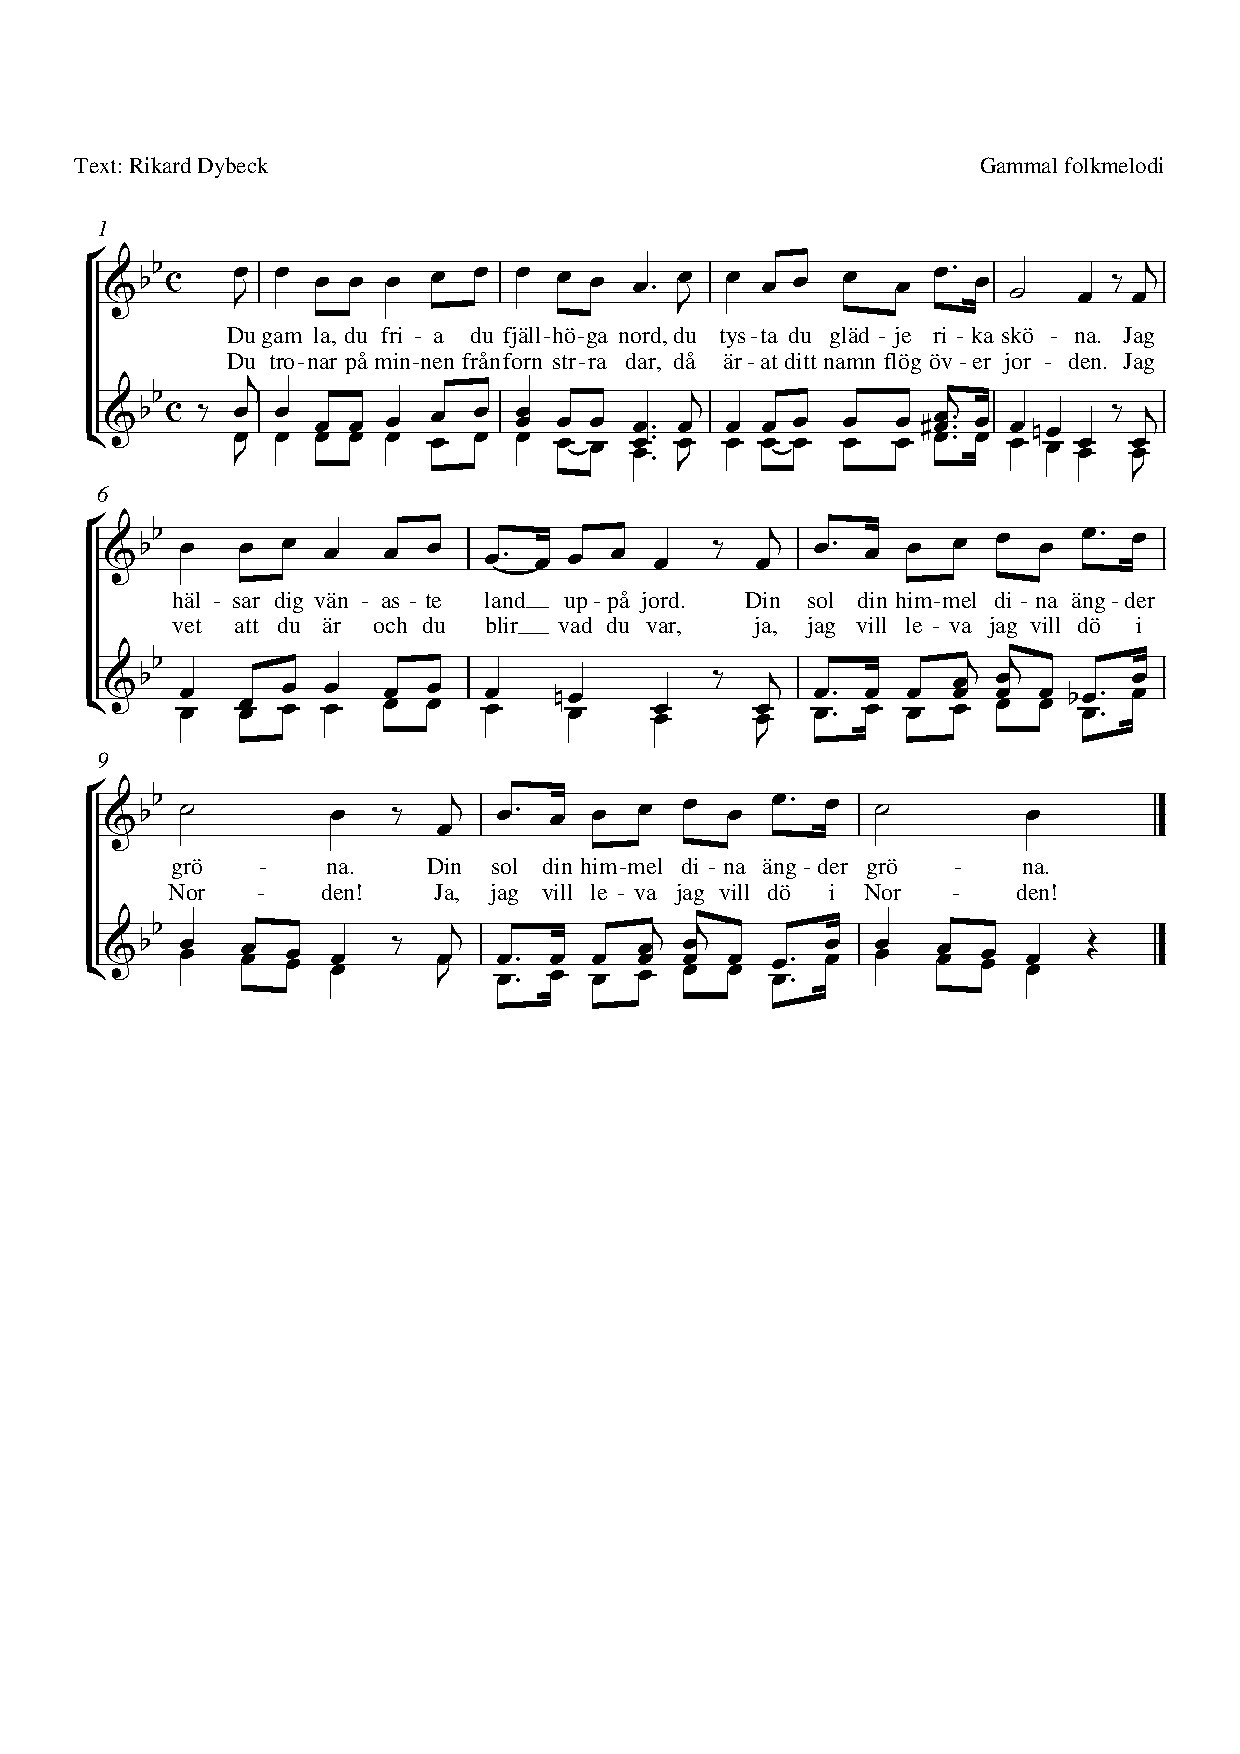
\includegraphics[width=\textwidth]{du_gamla_du_fria}
\end{figure}

\newpage
\setlength{\oddsidemargin}{-0.67in}
\begin{center}
\songtitle{$\omega2$}{Kungssången}
\end{center}
\vspace{-40pt}
\begin{figure}[!h]
\centering
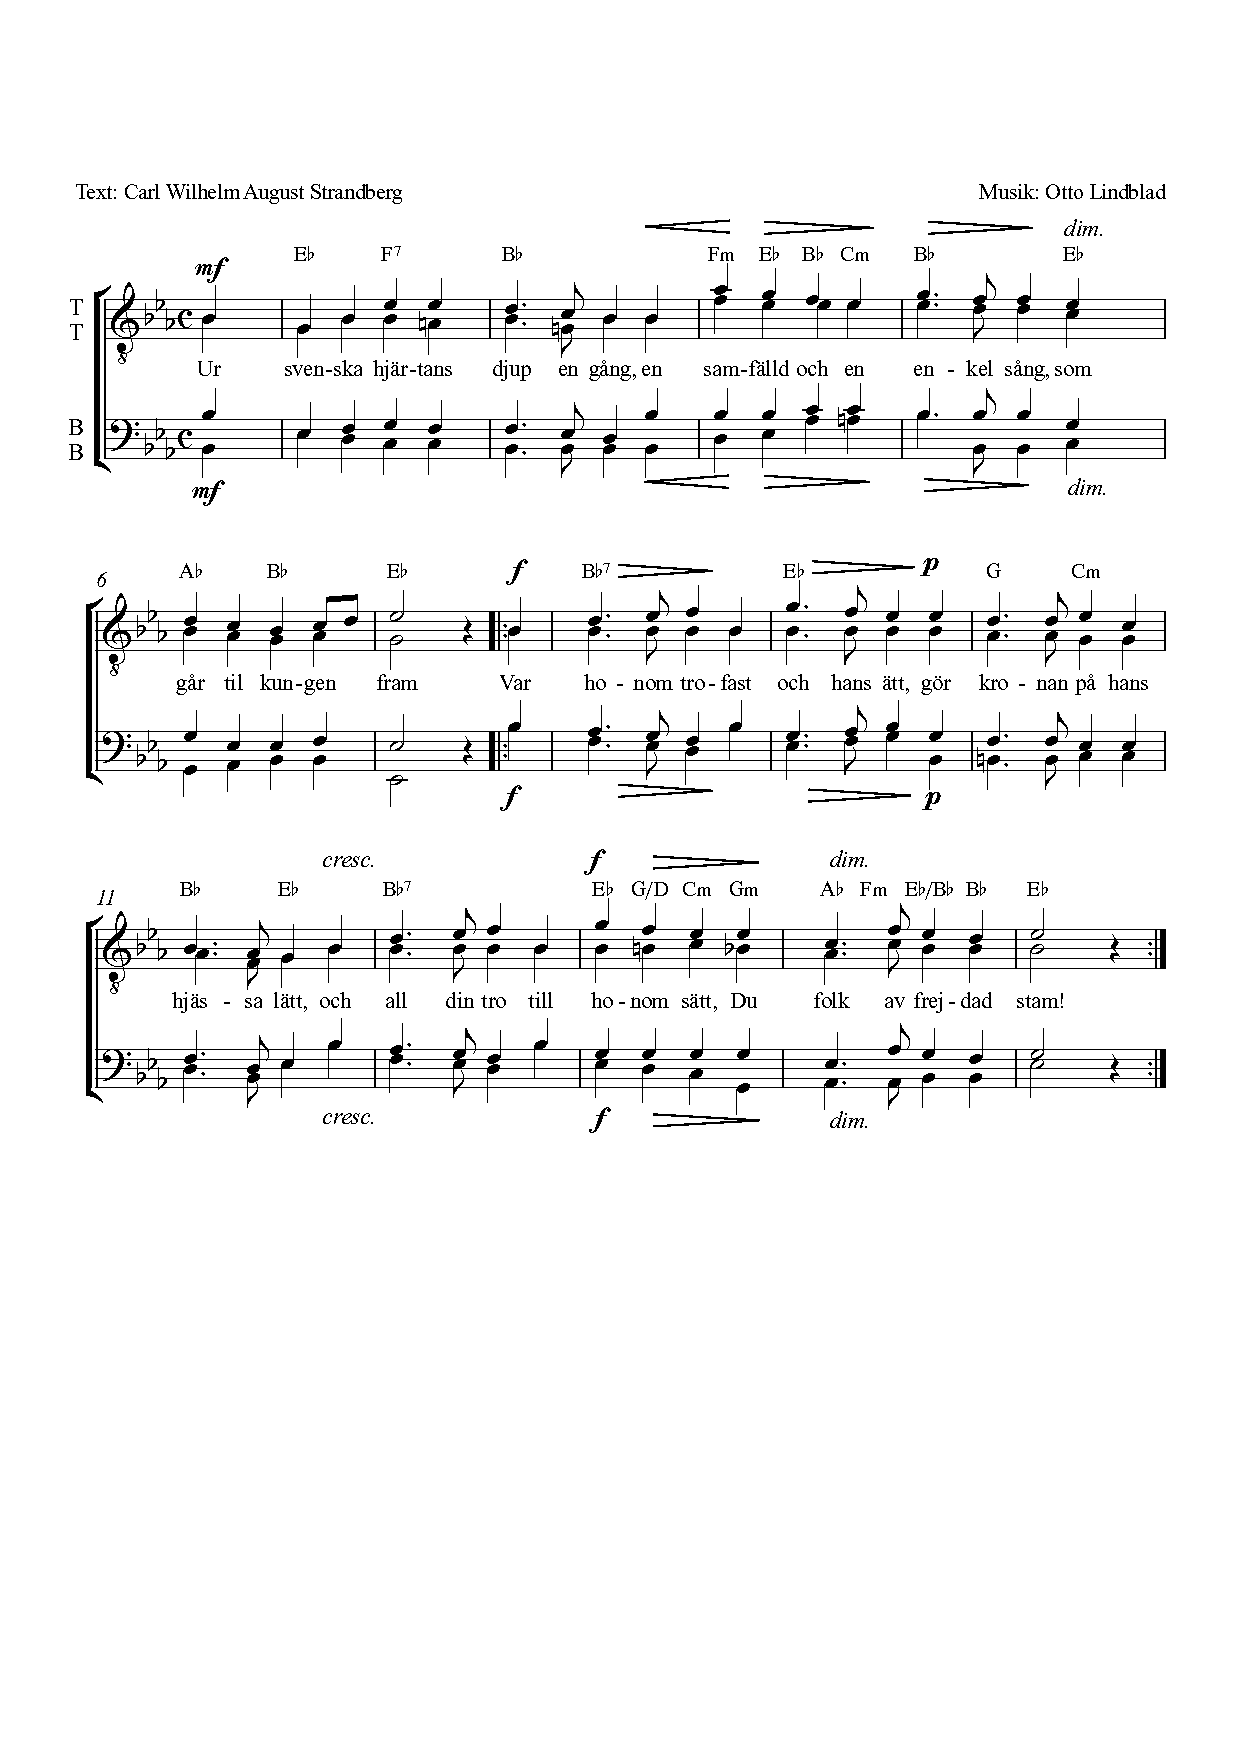
\includegraphics[width=\textwidth]{kungssangen}
\end{figure}

\newpage
\setlength{\oddsidemargin}{-0.47in}
\begin{center}
\songtitle{$\omega 3$}{Sveriges flagga}
\end{center}
\vspace{-40pt}
\begin{figure}[!h]
\centering
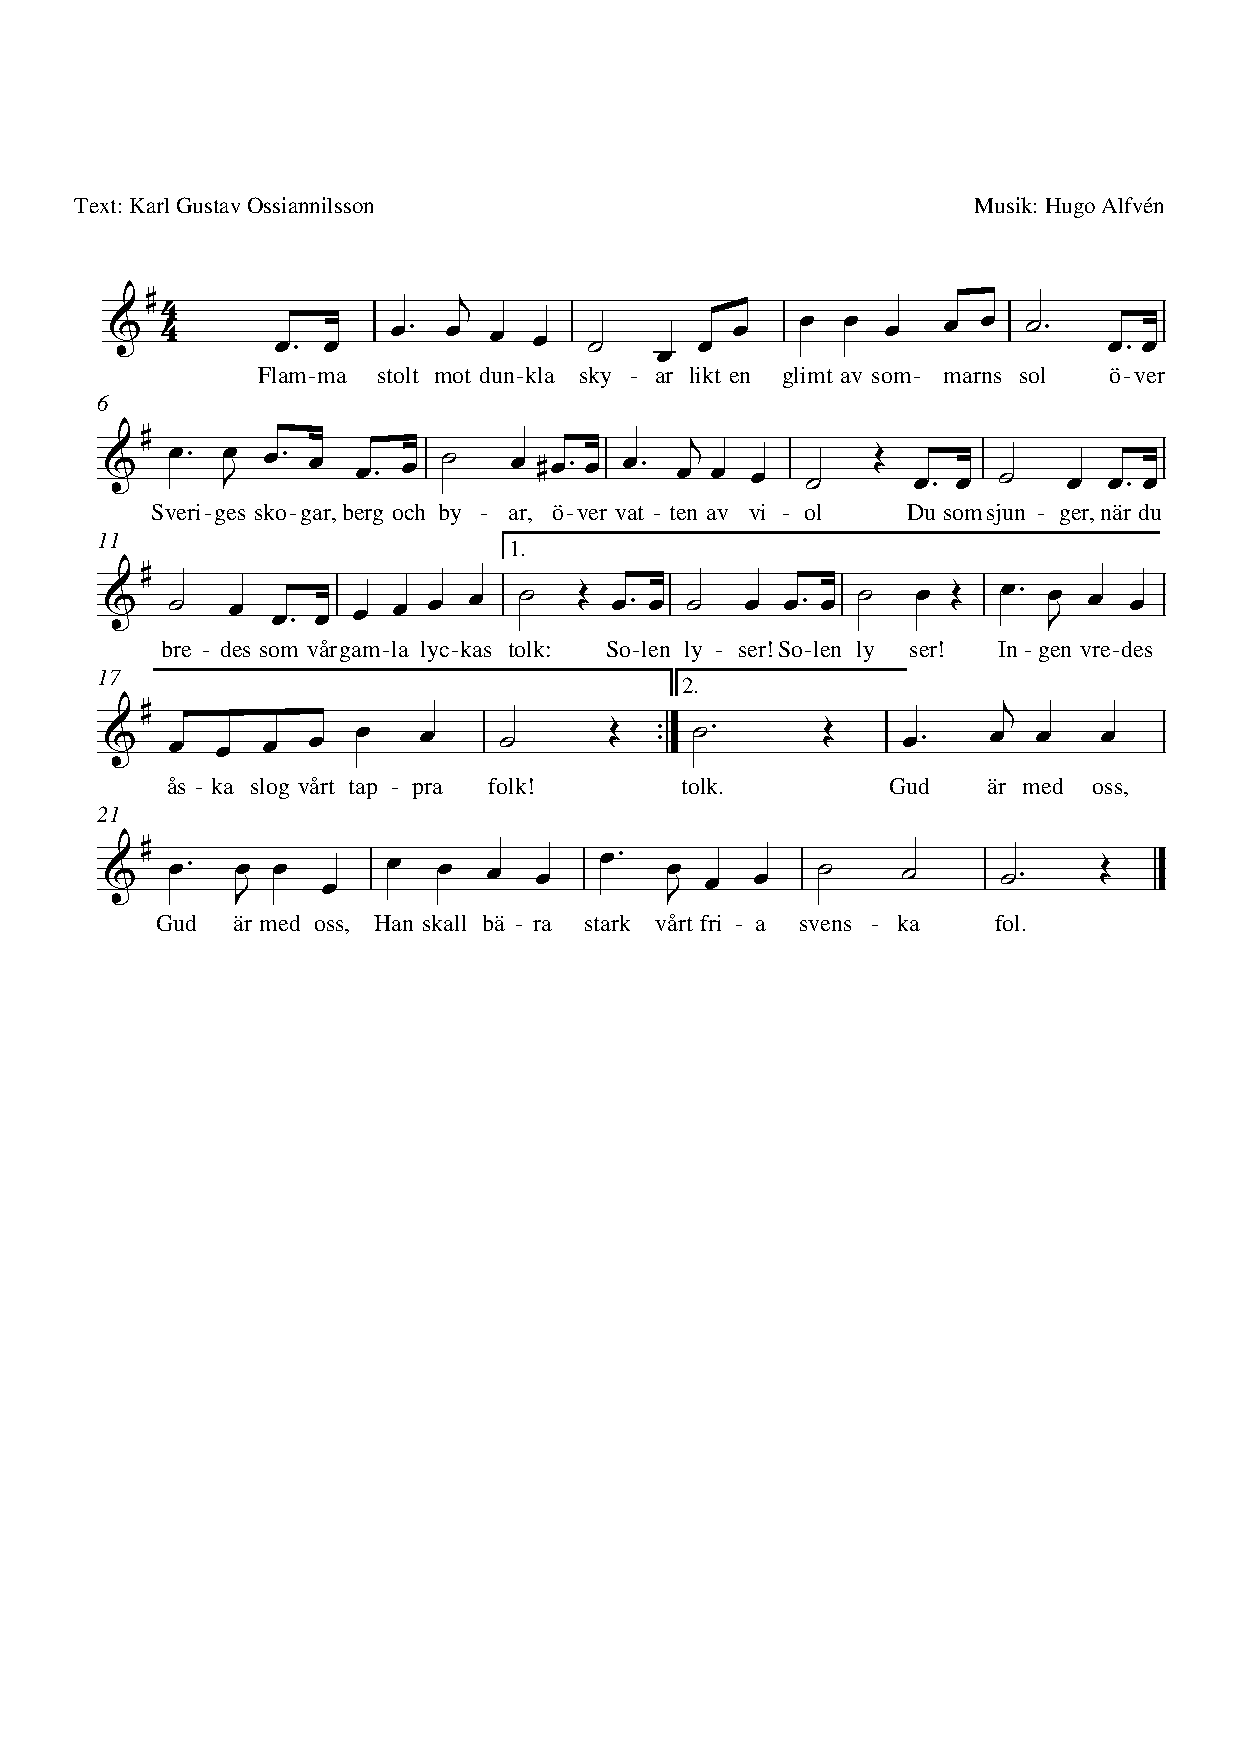
\includegraphics[width=\textwidth]{sveriges-flagga}
\end{figure}

\newpage
\setlength{\oddsidemargin}{-0.67in}
\begin{center}
\songtitle{$\omega4$}{Porthos visa}
\end{center}
\vspace{-40pt}
\begin{figure}[!h]
\centering
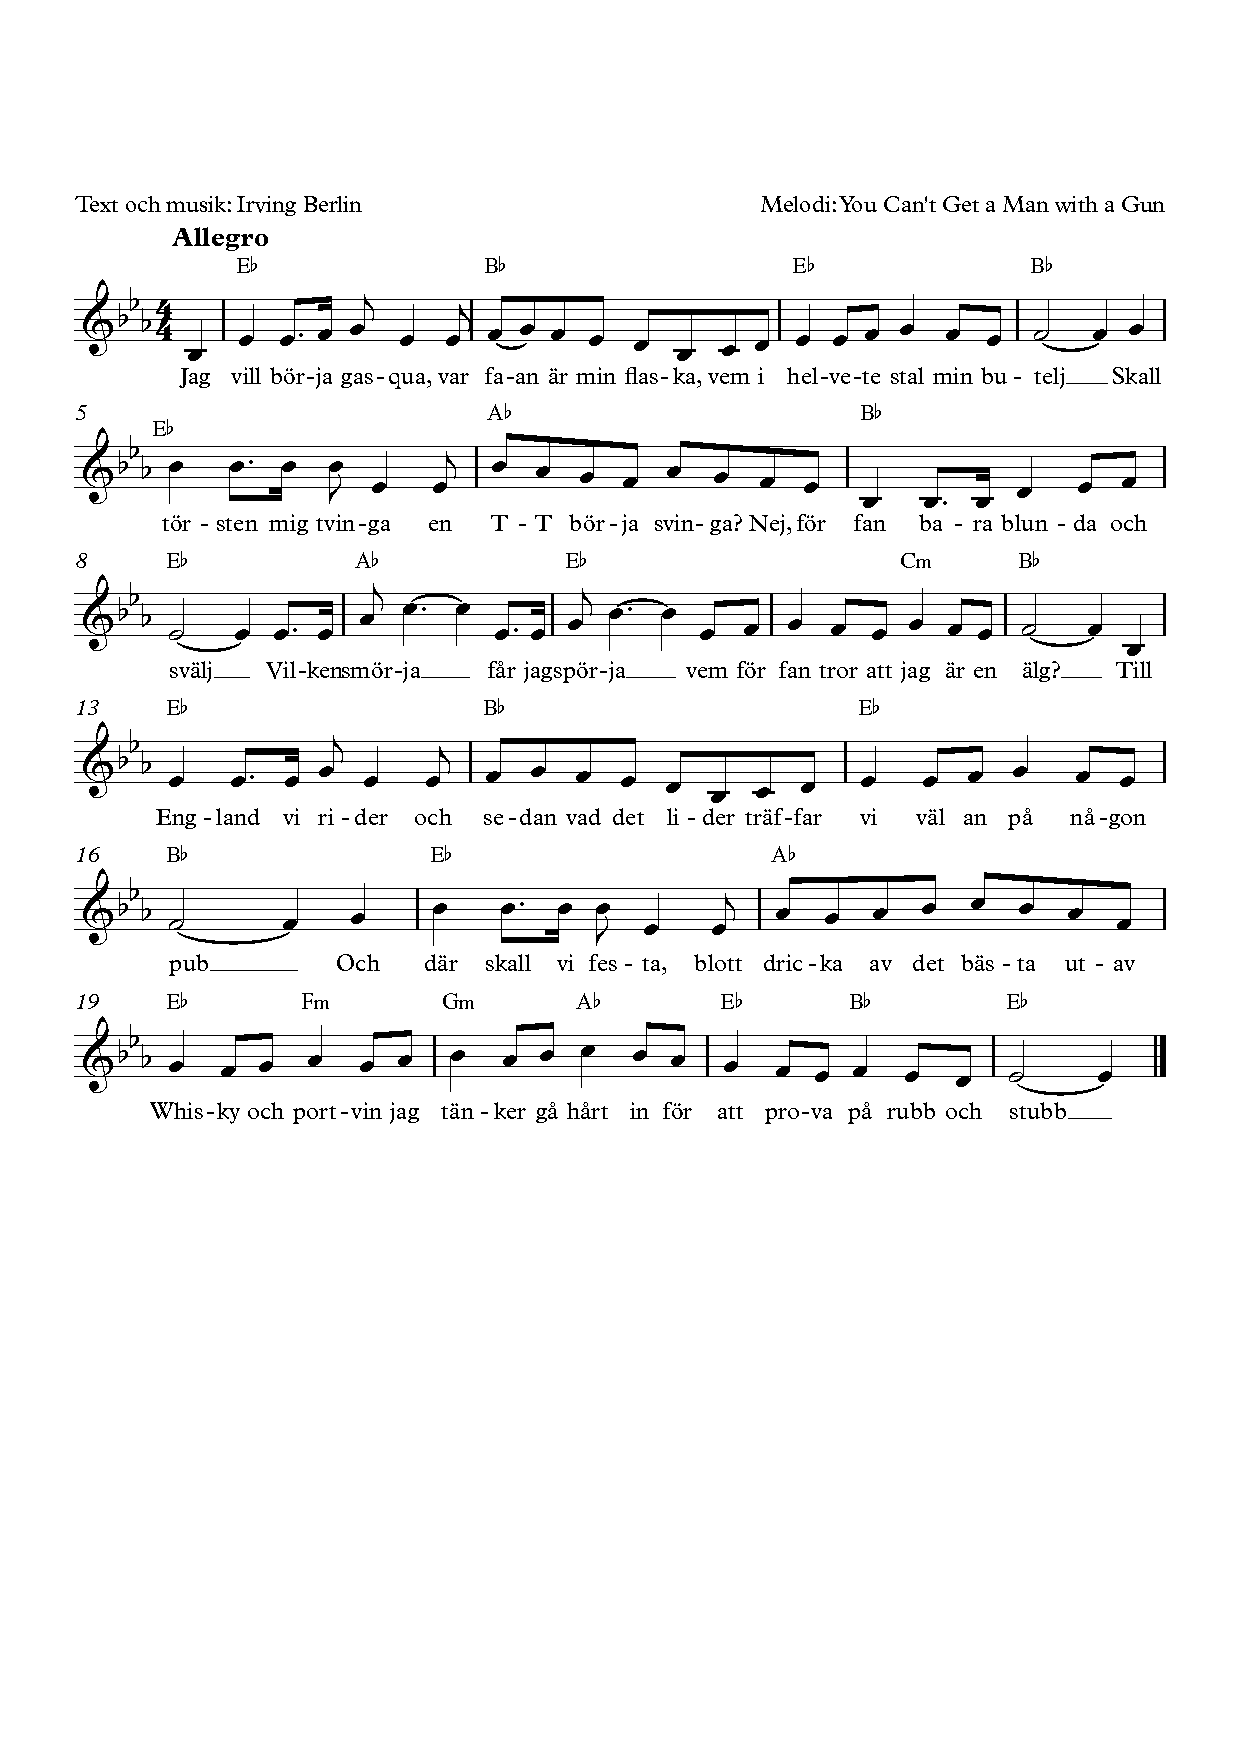
\includegraphics[width=\textwidth]{porthos}
\end{figure}

\newpage
\setlength{\oddsidemargin}{-0.47in}
\begin{center}
\songtitle{$\omega5$}{Lyft ditt välförsedda glas}
\end{center}
\vspace{-40pt}
\begin{figure}[!h]
\centering
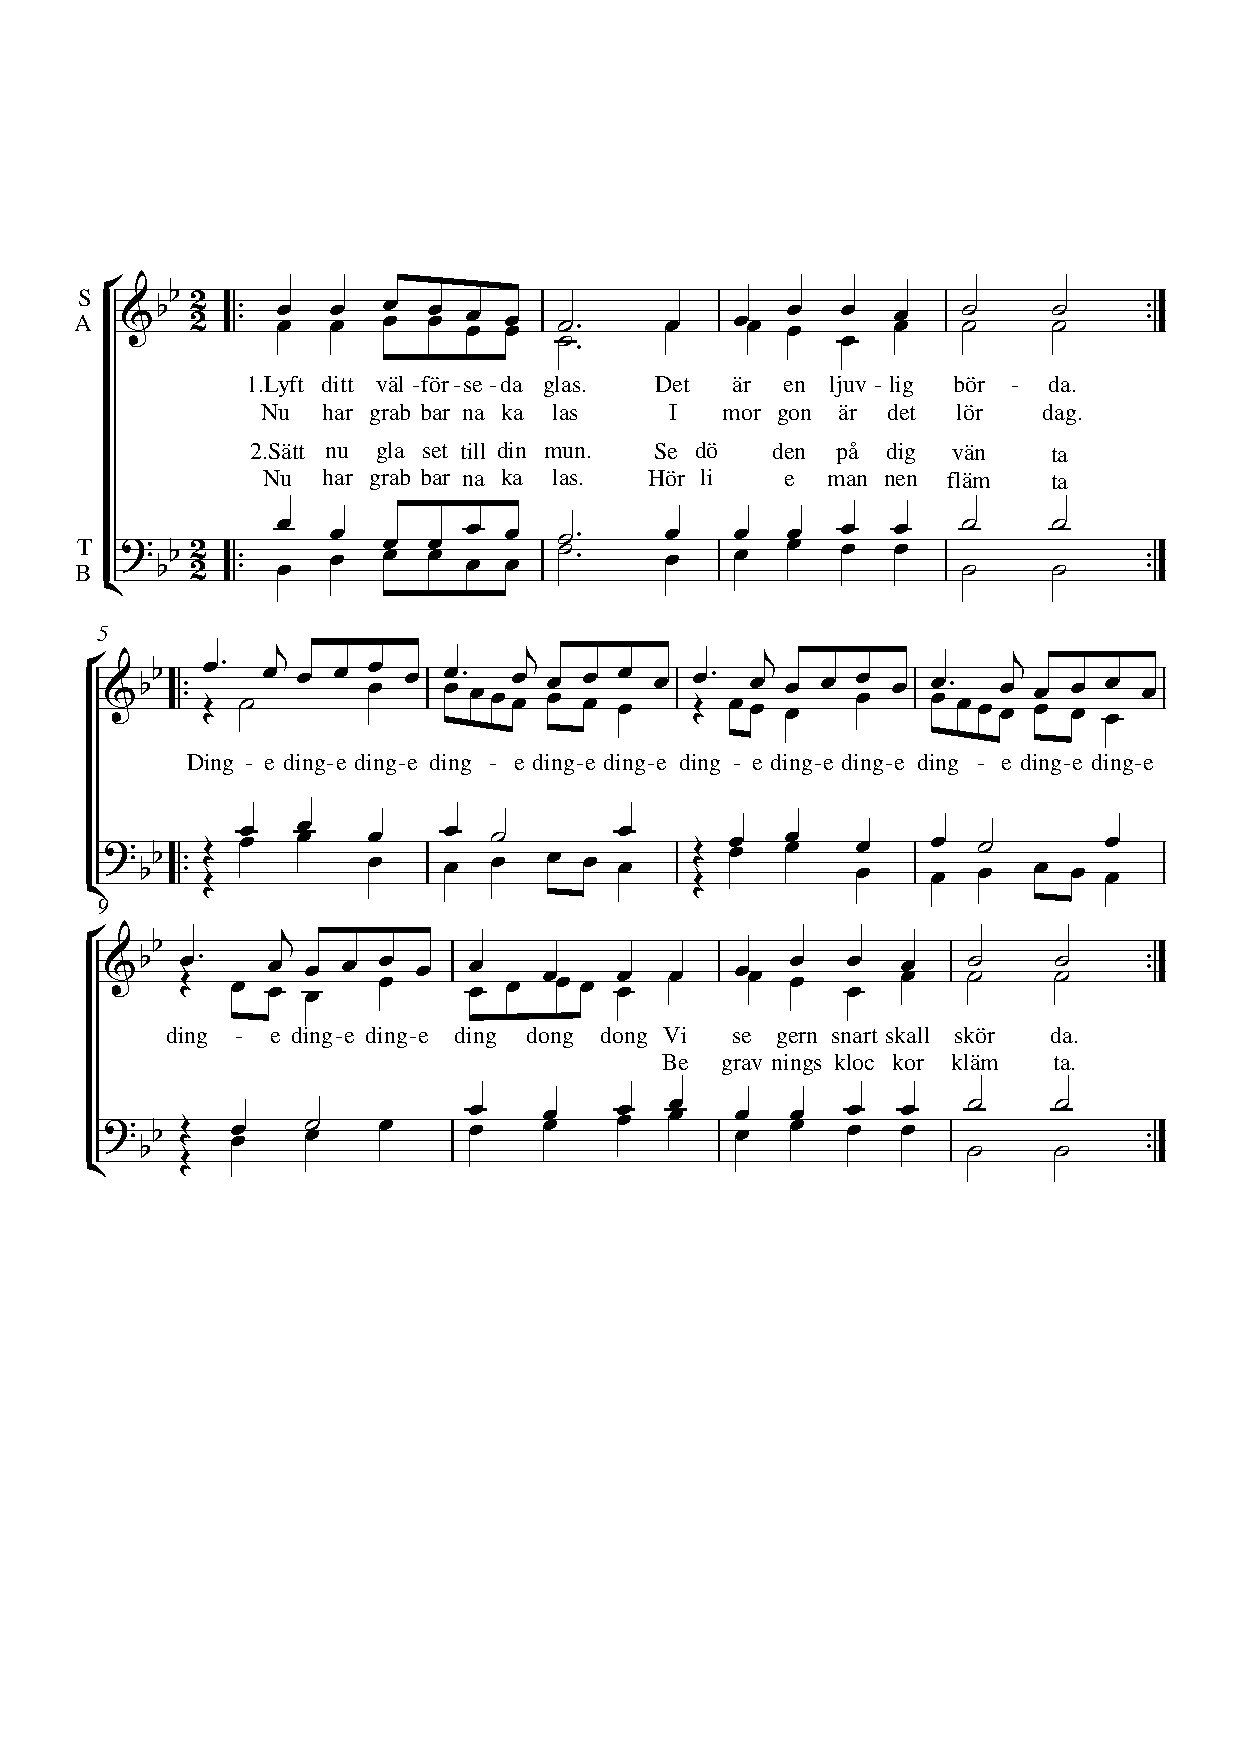
\includegraphics[width=\textwidth]{lyft-ditt-valforsedda}
\end{figure}

\newpage
\setlength{\oddsidemargin}{-0.67in}
\begin{center}
\songtitle{$\omega6$}{Längtan till landet}
\end{center}
\vspace{-40pt}
\begin{figure}[!h]
\centering
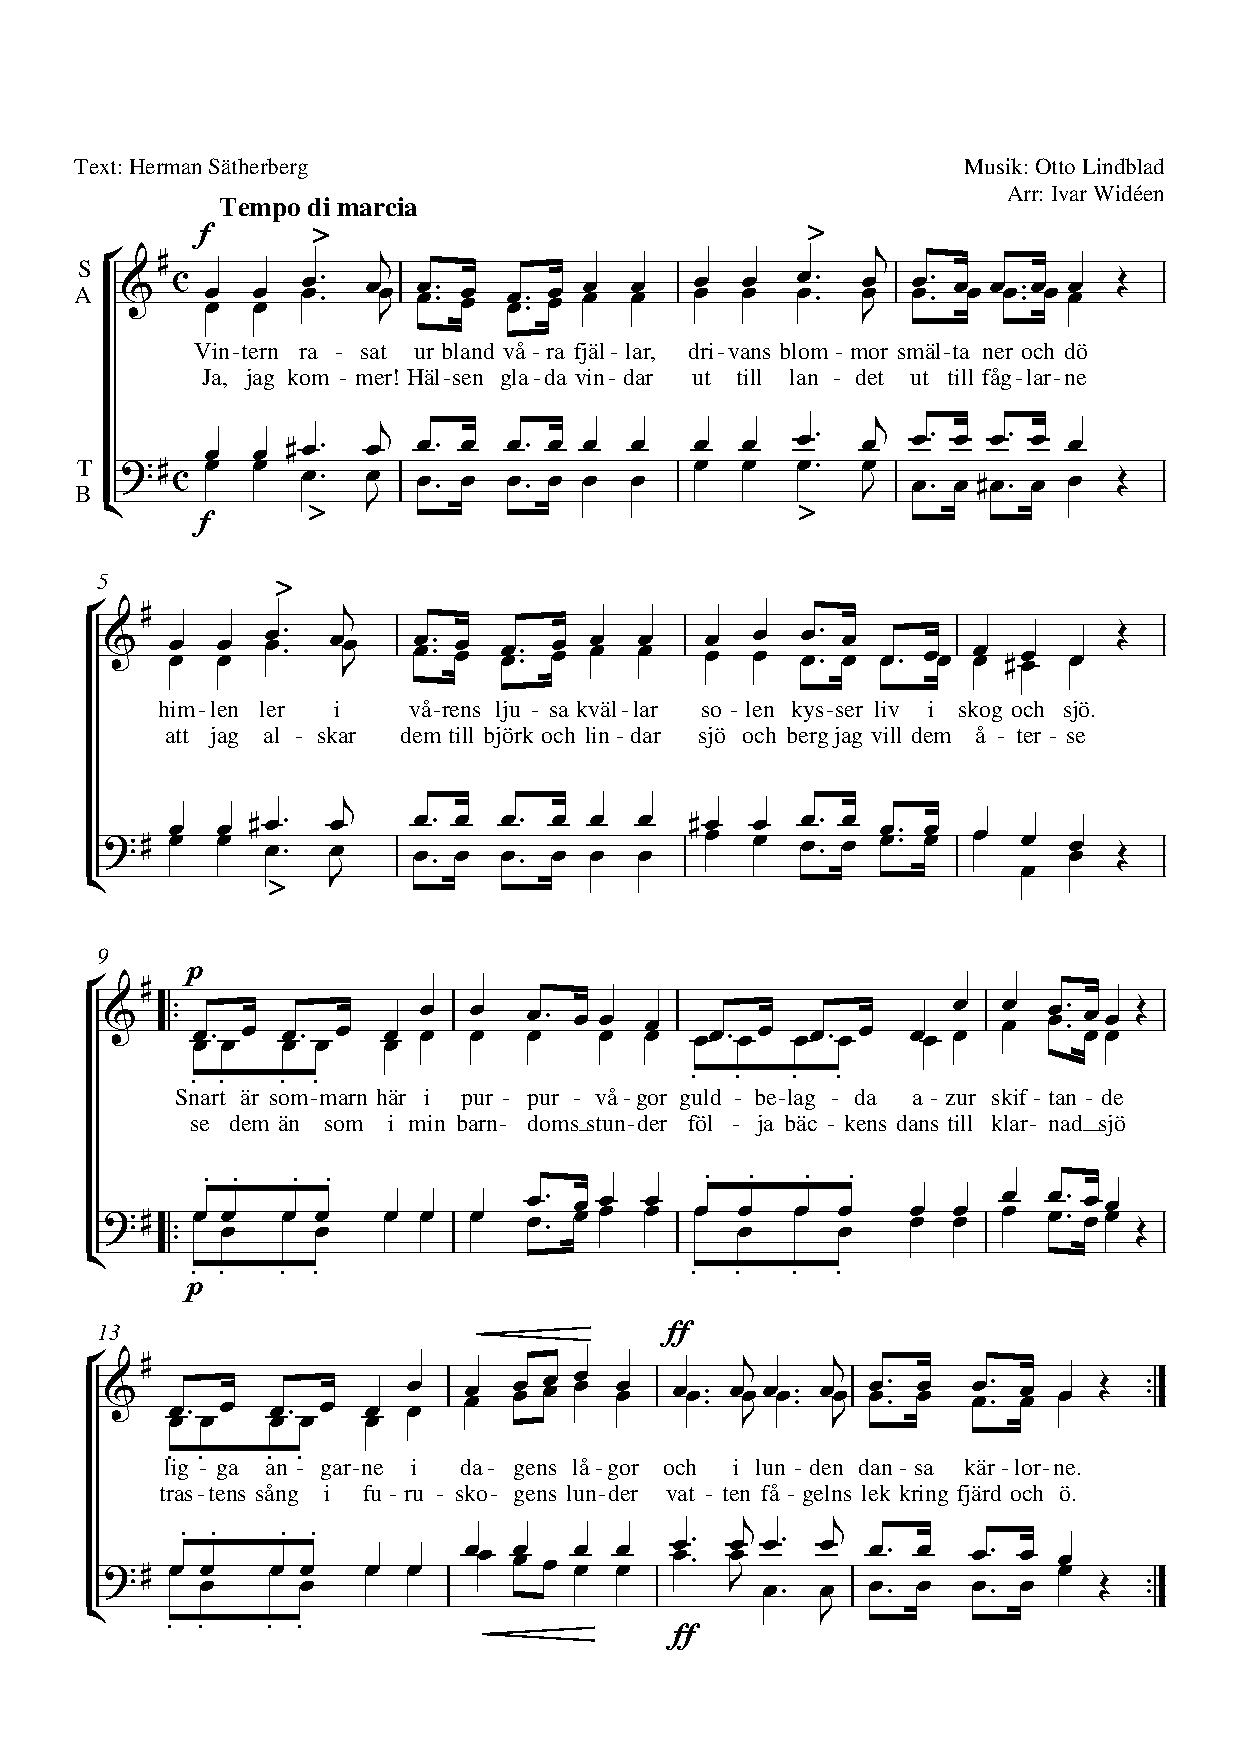
\includegraphics[width=\textwidth]{langtan-till-landet}
\end{figure}

\newpage
\setlength{\oddsidemargin}{-0.47in}
\begin{center}
\songtitle{$\omega7$}{Amanda Lundbom}
\end{center}
\vspace{-40pt}
\begin{figure}[!h]
\centering
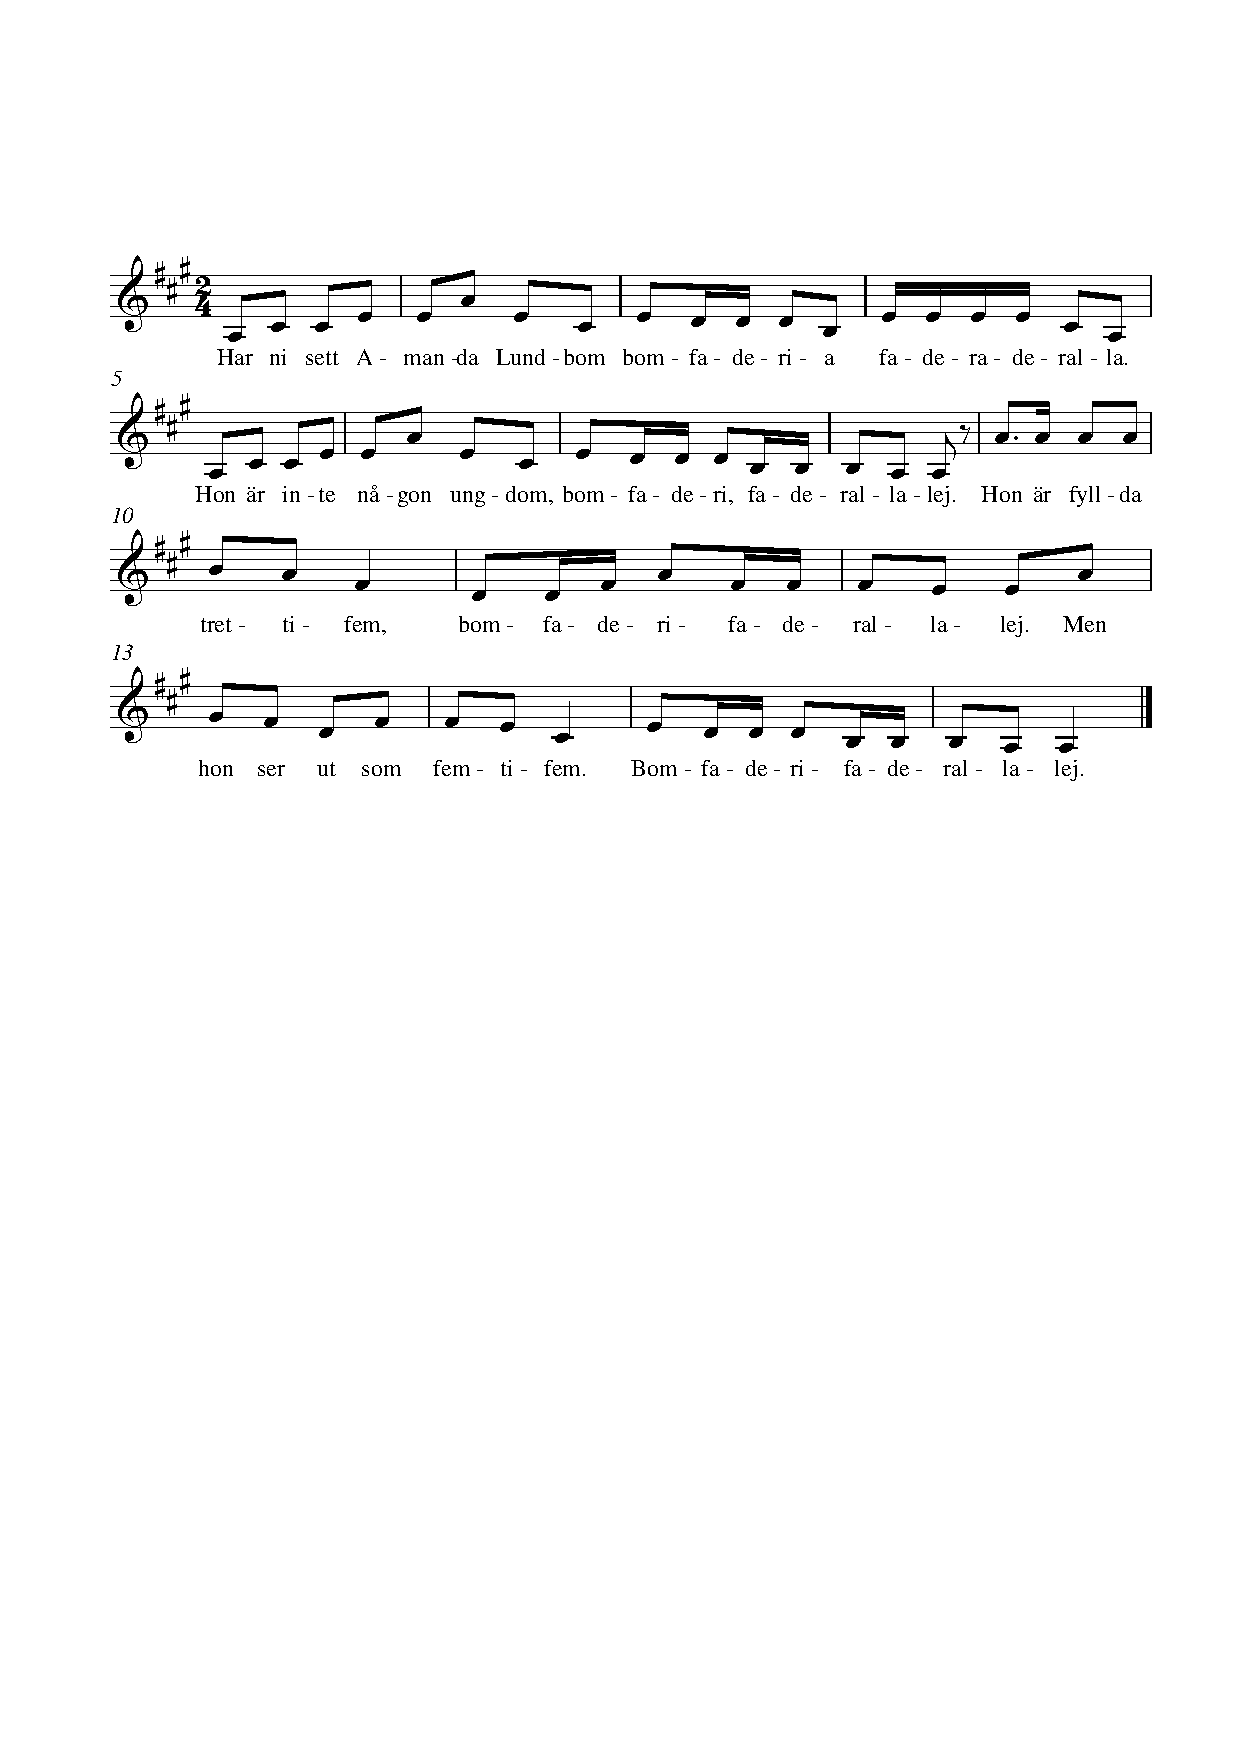
\includegraphics[width=\textwidth]{amandalundbom}
\end{figure}

\newpage
\setlength{\oddsidemargin}{-0.67in}
\begin{center}
\songtitle{$\omega8$}{Smedsvisa}
\end{center}
\vspace{-40pt}
\begin{figure}[!h]
\centering
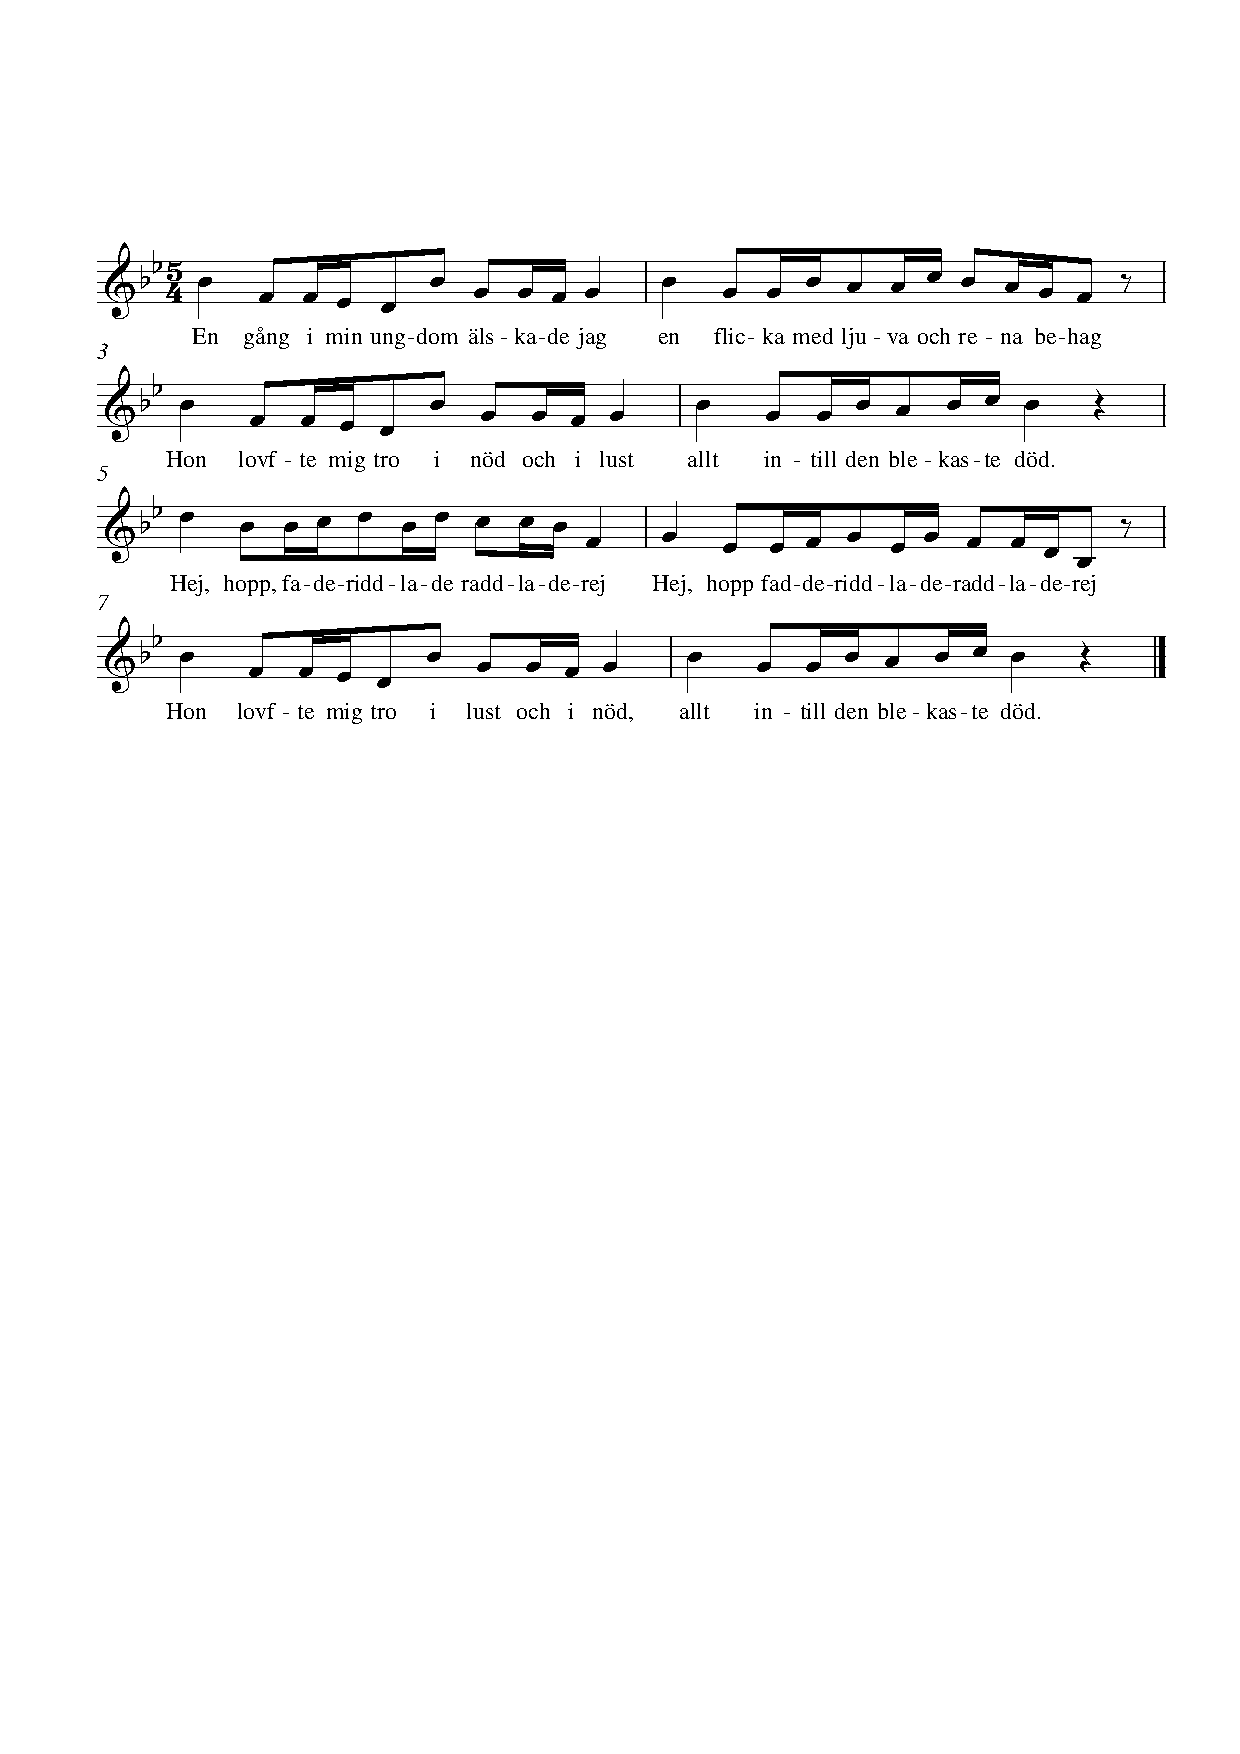
\includegraphics[width=\textwidth]{smedsvisa}
\end{figure}

\newpage
\setlength{\oddsidemargin}{-0.47in}
\begin{center}
\songtitle{$\omega9$}{Molltoner från Norrland}
\end{center}
\vspace{-40pt}
\begin{figure}[!h]
\centering
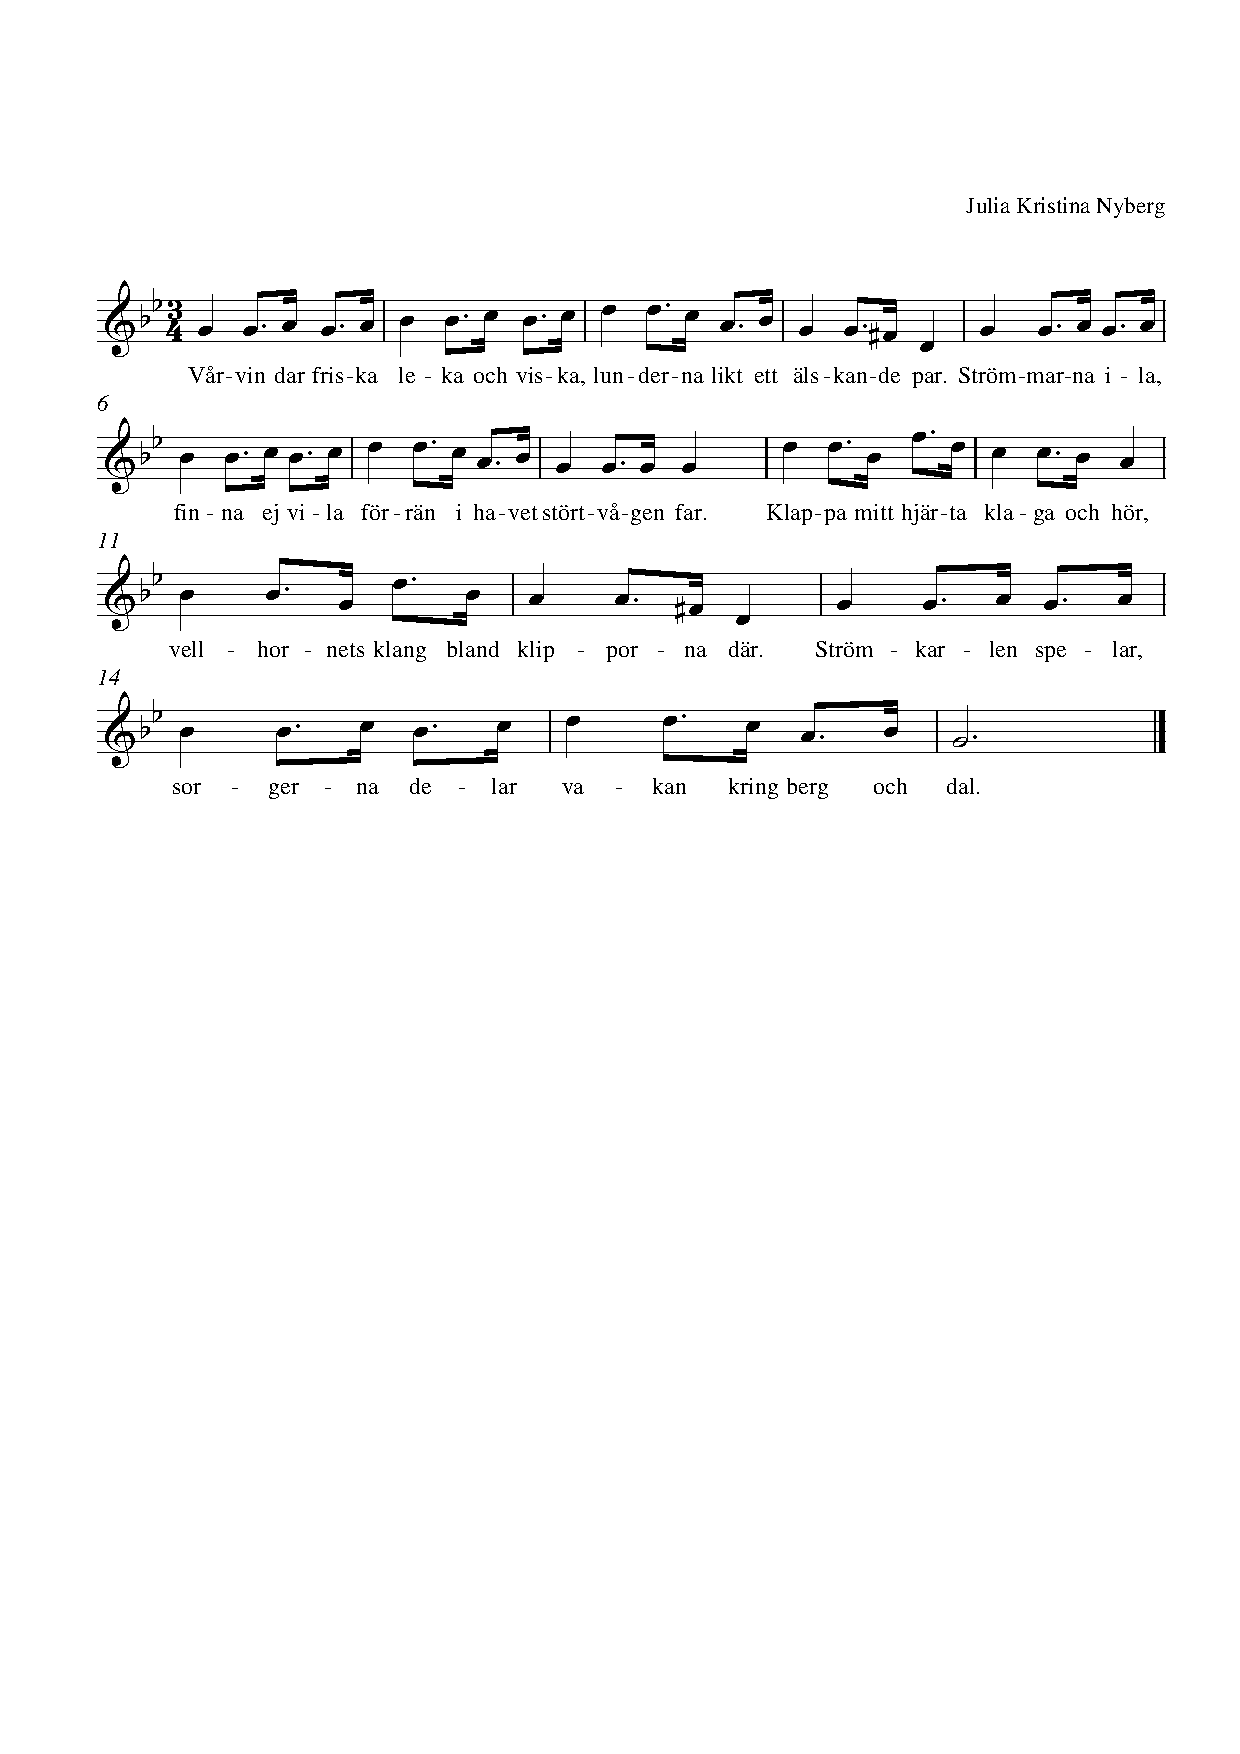
\includegraphics[width=\textwidth]{molltoner}
\end{figure}

\newpage
\setlength{\oddsidemargin}{-0.67in}
\begin{center}
\songtitle{$\omega10$}{Nu grönskar det}
\end{center}
\vspace{-40pt}
\begin{figure}[!h]
\centering
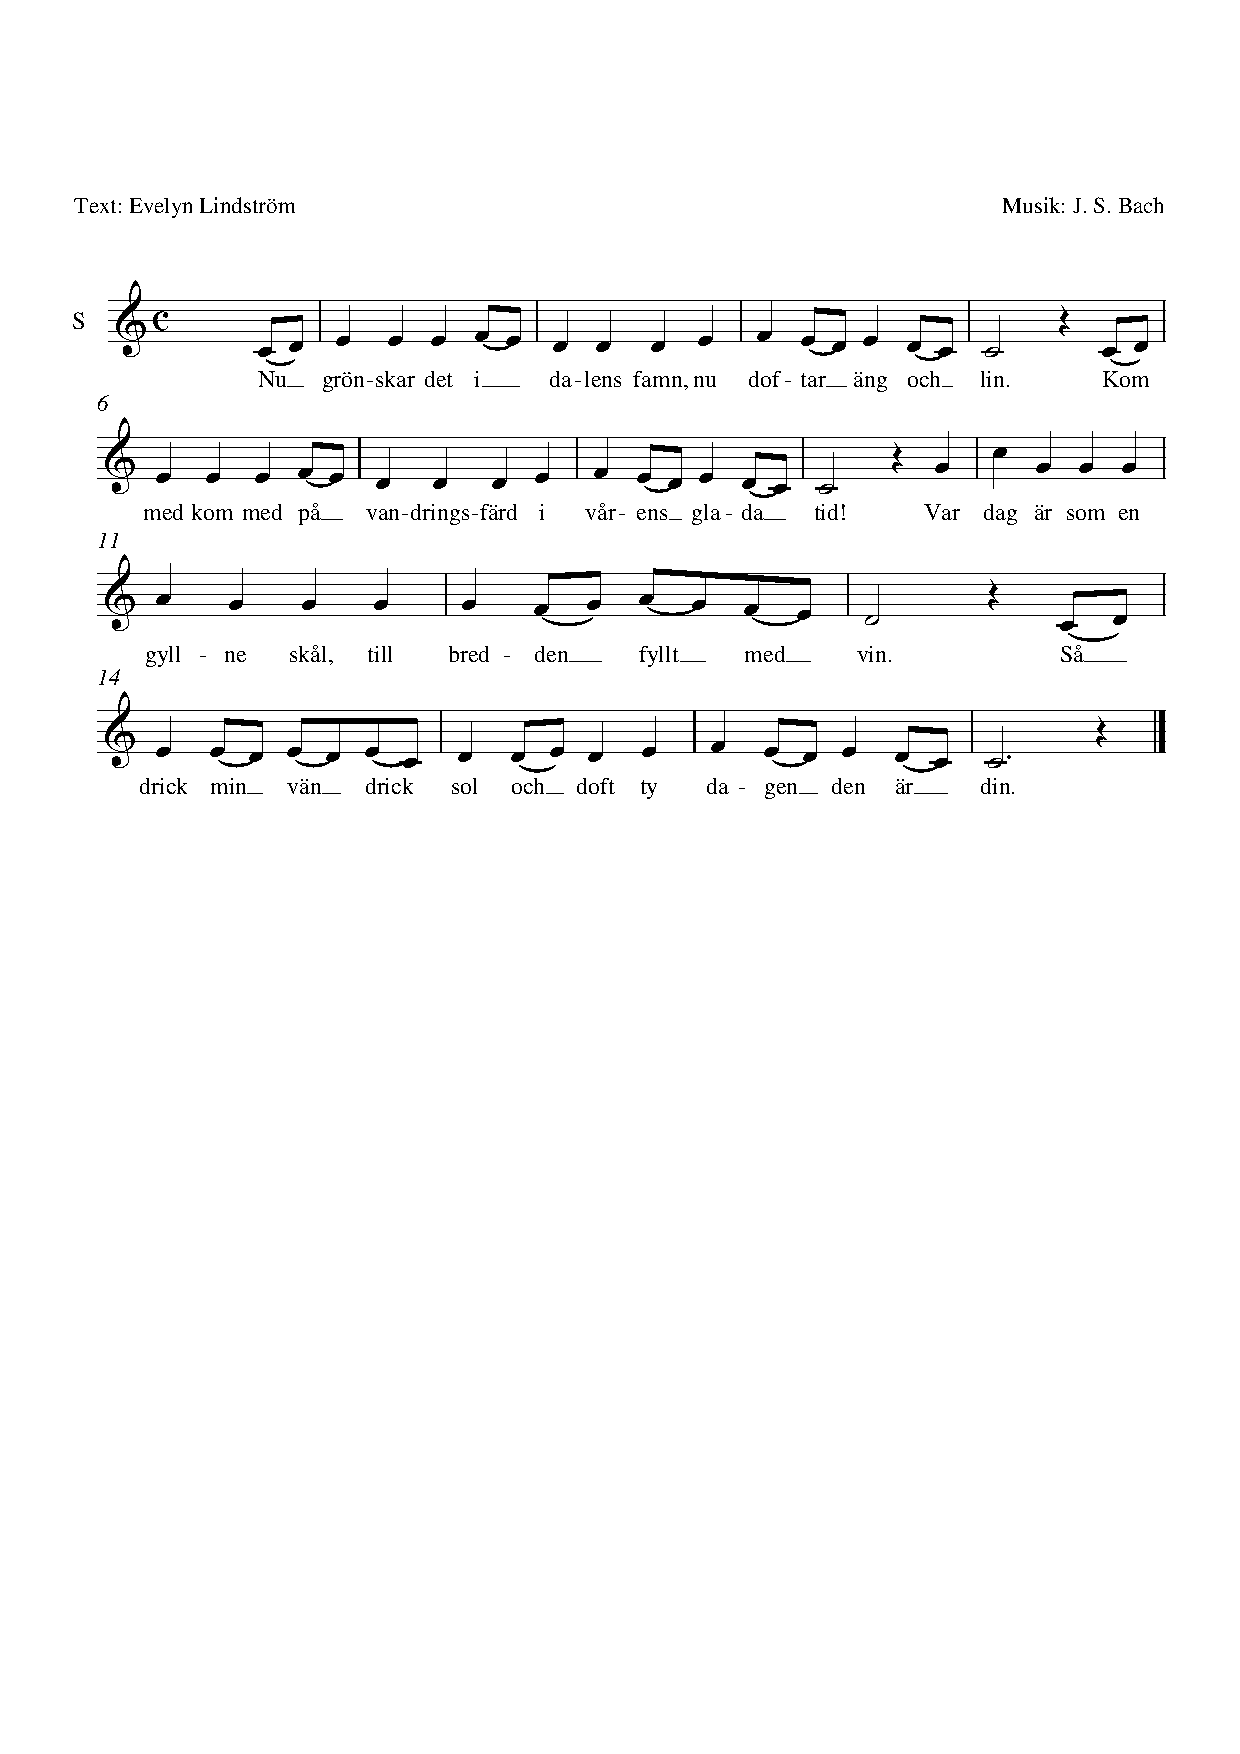
\includegraphics[width=\textwidth]{nugronskardet}
\end{figure}

\newpage
\setlength{\oddsidemargin}{-0.47in}
\begin{center}
\songtitle{$\omega11$}{Studentsången}
\end{center}
\vspace{-40pt}
\begin{figure}[!h]
\centering
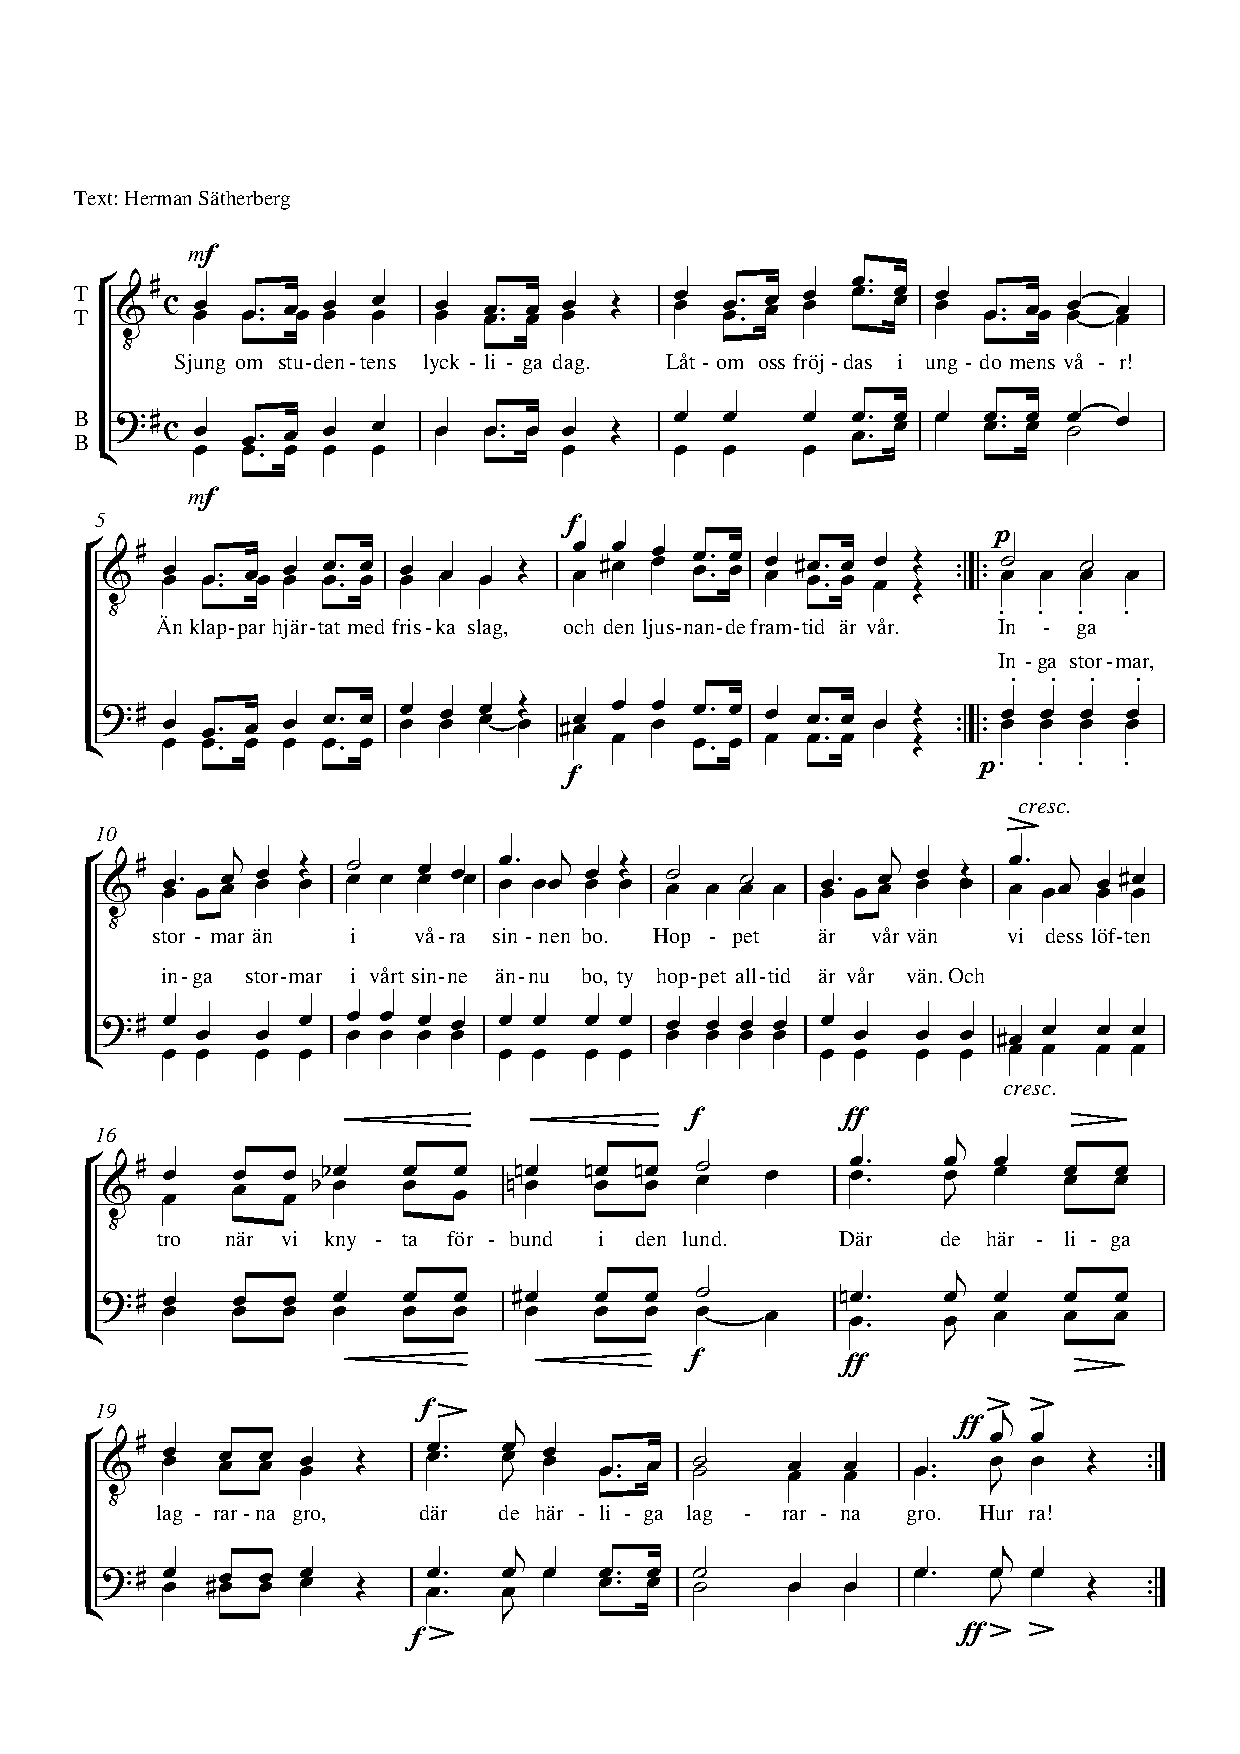
\includegraphics[width=\textwidth]{studentsangen}
\end{figure}

\newpage
\setlength{\oddsidemargin}{-0.67in}
\begin{center}
\songtitle{$\omega\infty$}{O gamla klang och jubeltid}
\end{center}
\vspace{-40pt}
\begin{figure}[!h]
\centering
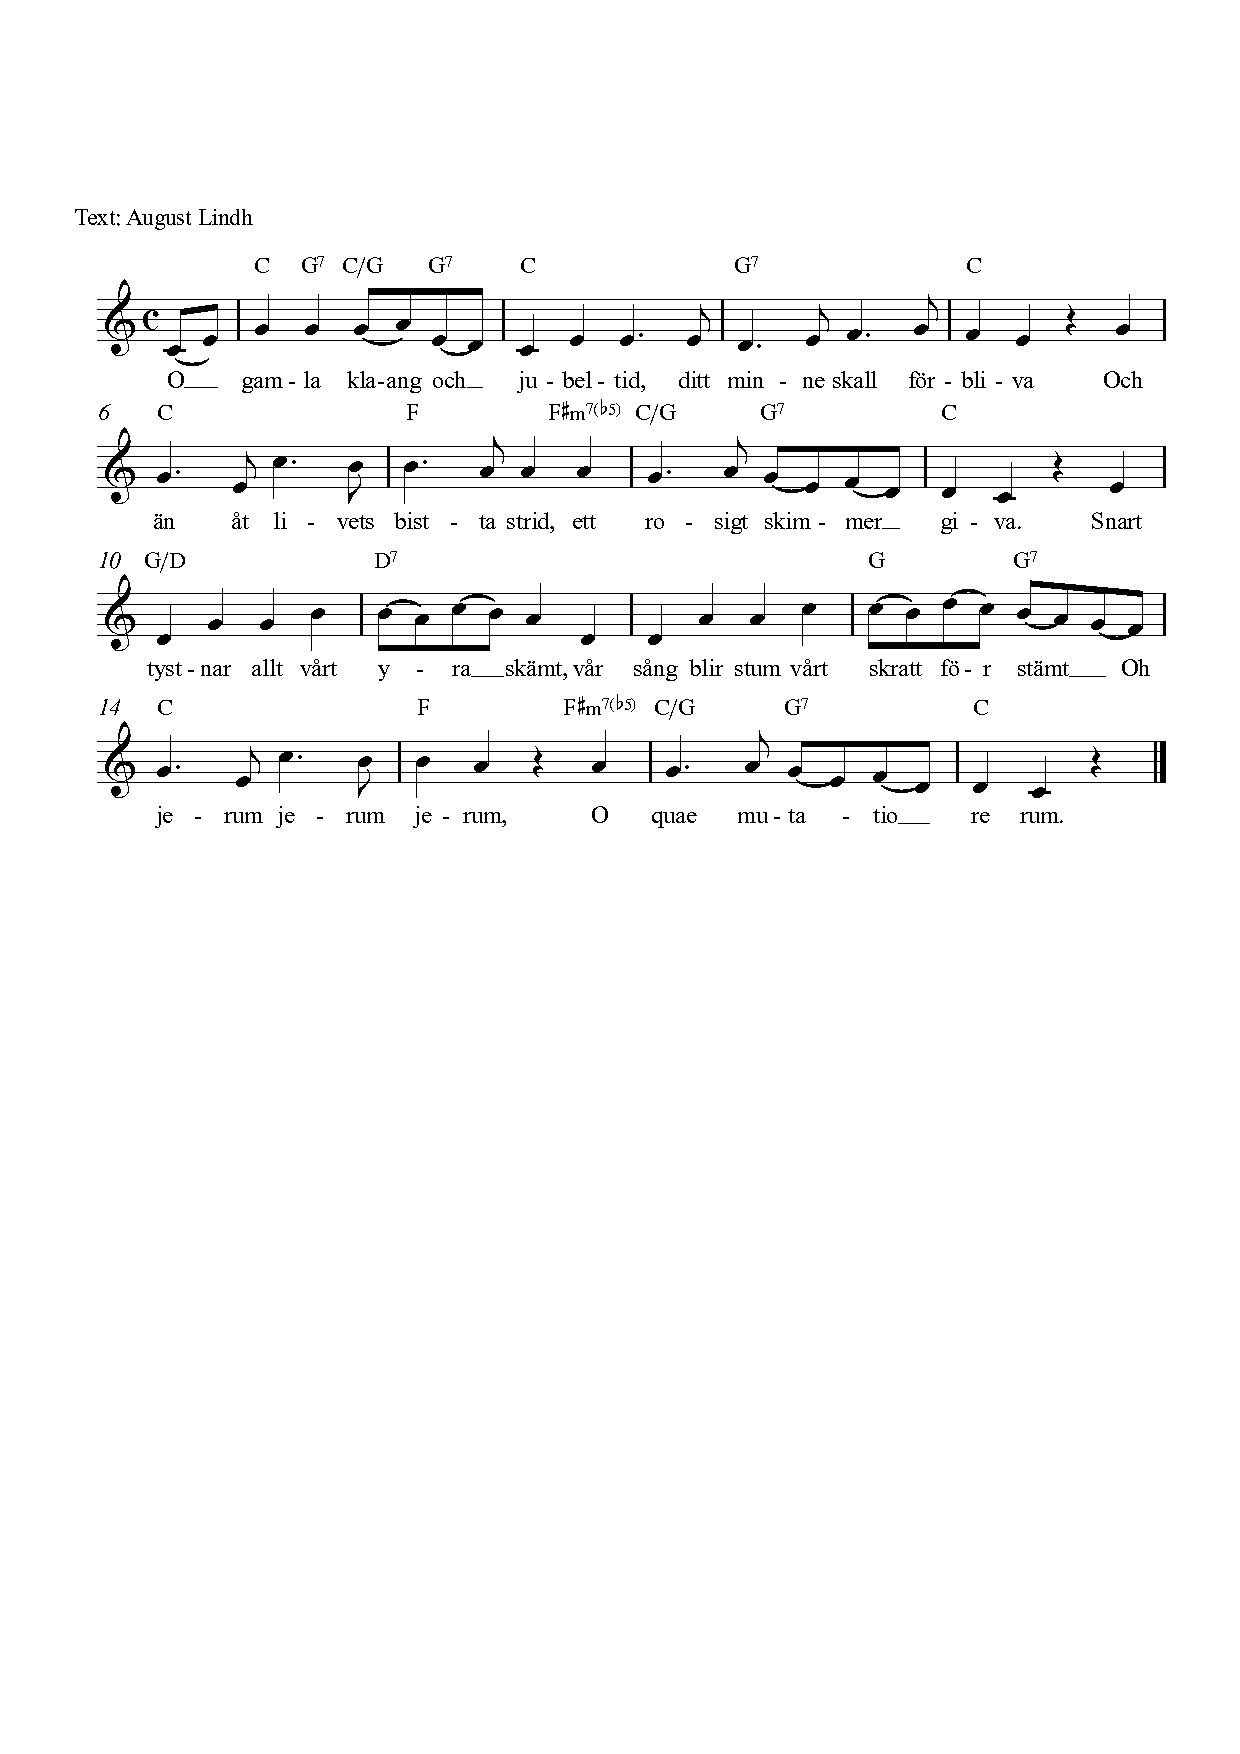
\includegraphics[width=\textwidth]{ogamlaklang}
\end{figure}
\end{document}